\chapter{Unscented Kalman Filters}
\label{Unscented Kalman Filters}

The Unscented Kalman Filter (UKF) is another nonlinear version of the Kalman Filter and was developed to address the shortcomings of the EKF. As opposed to using the Jacobian to linearly approximate around a single point, the UKF uses the Unscented Transform (UT) to approximate around multiple points, known as sigma points. The UT is a method of approximating probability distributions that have undergone a non linear transformation using limited statistics. The UT uses these sigma points, which are represented in a Sigma Point Matrix, to represent the normal distribution of the data. Then, the sigma points undergo a non-linear transformation, resulting in a posterior distribution that is not normal \cite{inbook, Wan01theunscented} . We are able to approximate the normal distribution of the posterior distribution using the weights and covariance that were calculated prior to the transformation. This process enables the Kalman Filter to be applied to more complex non linear problems. \\ \\

\noindent Unlike the Kalman Filter and the Extended Kalman Filter, the UKF also has a set of parameters. Explanations of each parameter and their default values can be found in Table 4.2. Here, parameters are necessary for controlling the spread of sigma points. This was not needed for the EKF, since the EKF was only linearizing around the mean. The thesis will not be exploring how to tune these parameters, but one method to do so is through ad hoc testing.

\begin{figure}[h]
    \centering
    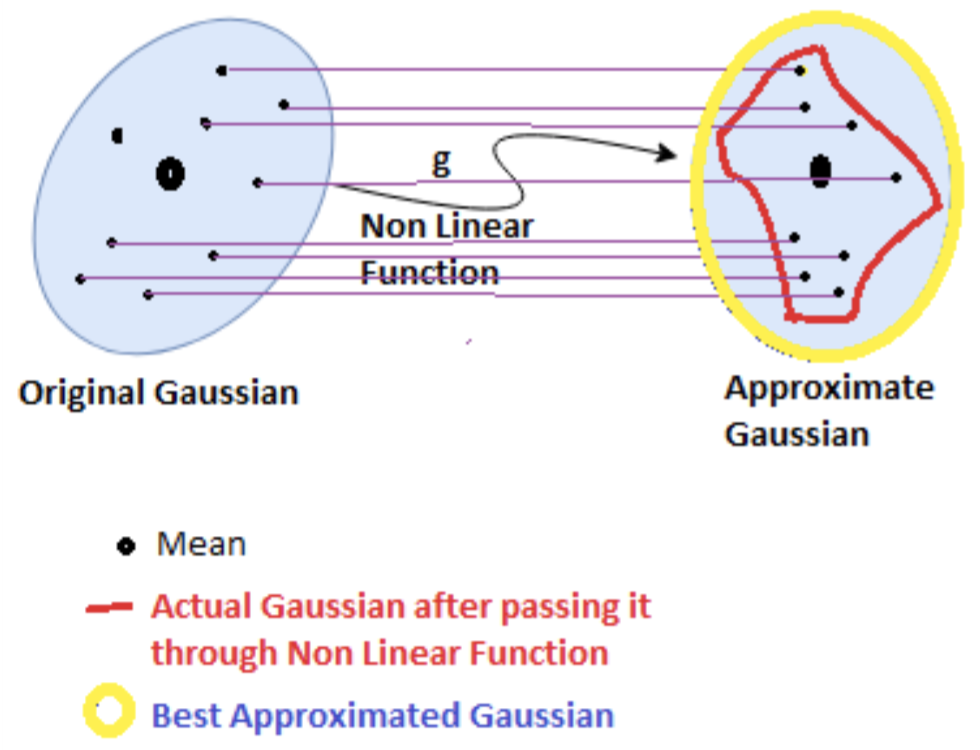
\includegraphics[scale = 0.7]{UKF.png}
    \caption{A depiction of the general overview of the UKF. Here we see that sigma points are sampled from a Gaussian distribution and are propagated through a non-linear function, called $g$. Though the output is non-Gaussian, an approximation of the Gaussian distribution can be obtained.}
\end{figure}

\newpage

\noindent The term 'unscented' was arbitrarily coined by the developer of the UKF, Jeffrey Uhlmann. In an interview, he shares:
\begin{displayquote}
"Initially I only referred to it as the “new filter.” Needing a more specific name, people in my lab began referring to it as the “Uhlmann filter,” which obviously isn’t a name that I could use, so I had to come up with an official term. One evening everyone else in the lab was at the Royal Opera House, and as I was working I noticed someone’s deodorant on a desk. The word “unscented” caught my eye as the perfect technical term. At first people in the lab thought it was absurd—which is okay because absurdity is my guiding principle—and that it wouldn’t catch on. My claim was that people simply accept technical terms as technical terms: for example, does anyone think about why a tree is called a tree?"
\end{displayquote}


\section{Unscented Kalman Filter Algorithm}
Before delving into the details of the algorithm, we will explore a high-level overview of the UKF process. As with the KF and the EKF, the UKF follows the three major components of:
\begin{enumerate}
  \item Initializing the model's states
  \item Generating a prediction
  \item Updating prediction with measurements from the system.
\end{enumerate}

\noindent In the first step, initializing the model requires calculation of sigma points. These sigma points characterize the normal distribution of the data. 
\begin{figure}[h]
    \centering
    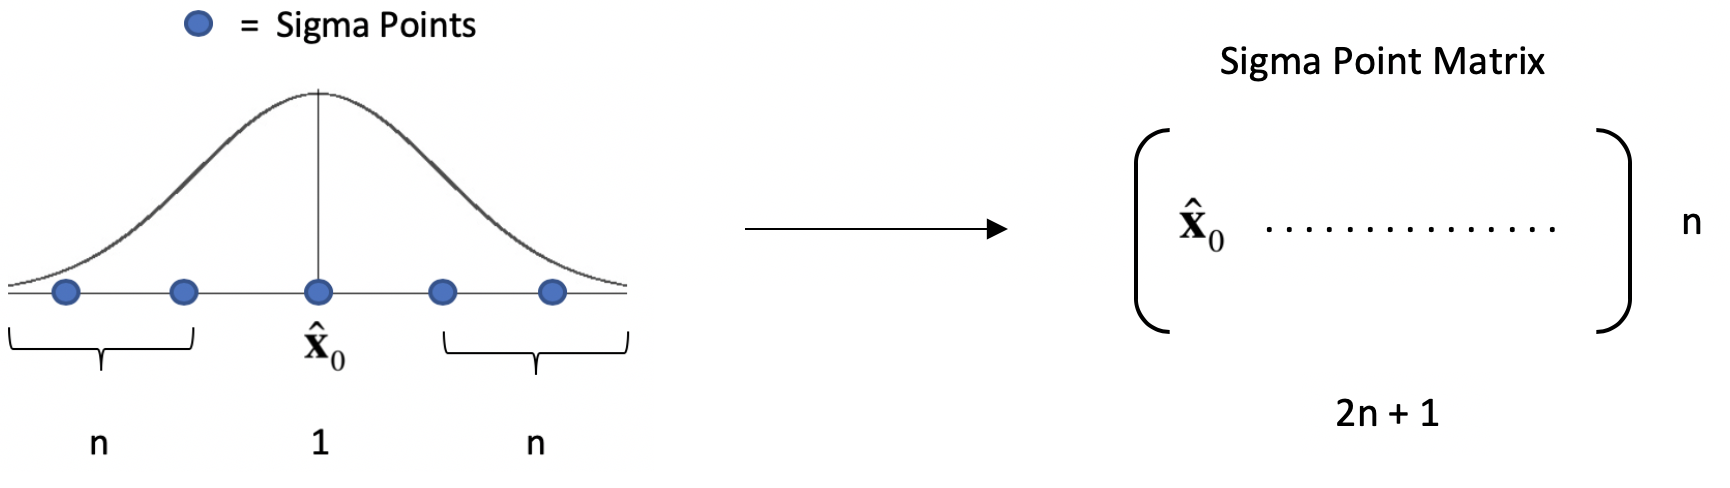
\includegraphics[scale = 0.4]{SPM.png}
    \caption{A brief illustration on how sigma points are used to characterize the Gaussian distribution of the data and how these sigma points are used to generate the Sigma Point Matrix.}
\end{figure}

\noindent After the sigma points undergo a nonlinear transformation, the resulting transformed sigma point matrix can be used to approximate the normal distribution of the data, which we can use to generate a prediction.
\begin{figure}[h]
    \centering
    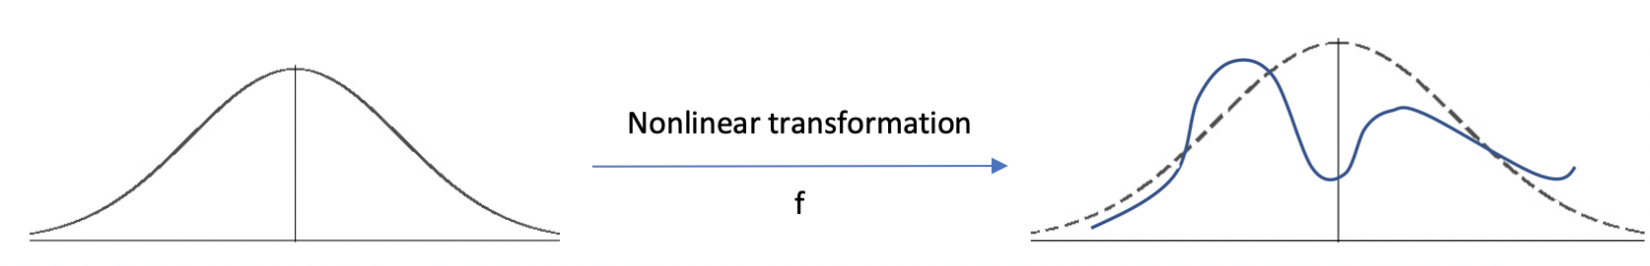
\includegraphics[scale = 0.45]{transform.png}
    \caption{After the Gaussian-distributed data undergoes a nonlinear transformation, call it $f$, the result is no longer linear}
\end{figure}

\newpage
\noindent One can see that this follows the basic outline of the previous versions of the KF, but the process of doing each step varies. More details about each step are explained below.

\begin{enumerate}
    \item The first step is to initialize state vector, $x_0$, and covariance, $P_{x_0}$, which is exactly similar to both the KF and the EKF. Since we know that the $x_0$ is normally distributed, the expectation can be calculated by
    \begin{align*}
    	x_0 = \mathbb{E}[x_0]   = \sum^n_{i = a} x_i p_i = [x_a p_a + x_b p_b + \hdots + x_n p_n]^T,
        %\hat{x}_{0} &= \mathbb{E}[x_{0}] 
    \end{align*}
   where $x_0= [x_a, x_b, \hdots, x_n]^T$, $p_a, p_b, \hdots, p_n$  is the respective probability of obtaining each state variable and $T$ is the transpose. Next initialize the state covariance, by
    \begin{align*}
        P_{x_{0}} &= \mathbb{E}[(x_{0}-\hat{x}_{0})(x_{0}-\hat{x}_{0})^{T}].
    \end{align*}
    
\noindent Unlike the KF and EKF, the UKF requires the calculation of sigma points, which is a way characterizing the distribution of the data. The number of sigma points is deterministic and depends on the dimensions of the system. In general, a UFK will have  $2x$ + 1 sigma points, where $x$ represents the dimension of the state vector \cite{inbook, inproceedings, Wan01theunscented}.  All sigma points are stored in a sigma point matrix, called $\chi$. To get a general idea about the distribution of the data, we use $\lambda$, which is a scalar value that determines how spread out the sigma points are from the mean. $\lambda$ can be calculated by
         \begin{align*}
        \lambda = \alpha^{2}(\text{x}+\kappa)-x,
         \end{align*}
         where x is a scalar representing the number of states in the system, and $\alpha$ and $\kappa$ are both parameters that control for the spread of sigma points around the mean value of the state. The spread of the sigma points is proportional to $\alpha$. For both $\alpha$ and $\kappa $,  the smaller the values are, the closer the sigma points are to the mean.\\ \\
       Another parameter of the UKF is $\beta$, which uses information regarding state distribution to adjust sigma points. $\beta$ has a default value of 2 if the data is Gaussian (which is an assumption we will make throughout this paper).  \\ \\
       Since the goal of this step is to characterize the distribution, set one of these sigma points to the mean, $\chi_{\ 0,k-1}$ which can be expressed as 
    \begin{align*}
        \chi_{\ 0,k-1} &= x_{k-1|k-1} ,
     \end{align*}
     where 0 is a row on $\chi$ and $k-1$ is the time step. Then allocate half of the remaining points will be smaller than the mean and the other half will be larger than the mean by
         \begin{align*}
        \chi_{\ i,k-1} &= x_{k-1|k-1} +  \bigg(\sqrt{(x+\lambda )P_{x,{k-1}}}\bigg)_{i} \quad \quad \quad i=1,\dots, x, 
        \end{align*}
         \begin{align*}
        \chi_{\ i,k-1} &= x_{k-1|k-1} - \bigg(\sqrt{(x+\lambda )P_{x_{k-1}}}\bigg)_{i-n} \quad \quad \quad i=x + 1,\dots,2x + 1,
        \end{align*}
        where x is the dimension of the state vector, $(\sqrt{(d_{x}+\lambda)P_{x_{k-1}}})$ is a matrix, and the $i$ subscript is the $i^{th}$ column of the matrix. 
        Recall that the square root of a matrix, satisfies the following condition: $A = B^2$, where $A$ and $B$ are both matrices. 
        
        
\noindent Next, we must calculate a weight for each sigma point. Weights are scalars used to calculate posterior sigma points after they have undergone a nonlinear transformation. One set of weights,  $W^{(m)}$, will be used to calculate the posterior mean while another set of weights $W^{(c)}$ will be used to calculate the posterior covariance. Weights can have positive or negative values, but will ultimately sum to 1 \cite{article6}. \\
        
\noindent The initialized weight for the mean, $W^{(m)}_{0} $ can be found by
            \begin{align*}
        W^{(m)}_{0} = \frac{\lambda}{x+ \lambda},
         \end{align*}
         where x is the number of states in the system. Similarly, the weight for the covariance at the initial time step, $W^{(c)}_{0}$, is given by
        \begin{align*}
        W^{(c)}_{0} = \frac{\lambda}{x+ \lambda} + (1 - \alpha^{2} + \beta).
         \end{align*}
          In later time steps, $W^{(m)}_{i} $ and $W^{(c)}_{i}$ follow the same equation, given by
               \begin{align*}
        W^{(m)}_{i} = W^{(c)}_{i} = \frac{\lambda}{2(x + \lambda) } \quad \quad \quad i=1,\dots,2x.
            \end{align*}
           
          
           
        \item A prediction can be generated by performing a nonlinear transformation on the sigma point matrix, $\chi$, in order to generate a prediction and provide an update on the covariance matrix. After $\chi$ undergoes a nonlinear transformation, $f$, the result is a transformed sigma point matrix at time step $k$ given the last time step, $k-1$, which will is called $\chi_{k | k - 1}$ and is given by
        \begin{align*}
        \chi_{k | k - 1} = f(\chi).
        \end{align*}
        
        
        Though $\chi$ has a Gaussian distribution,  $ \chi_{k | k - 1} $ does not because it has been transformed by the nonlinear state function $f$. The sum of the columns in $ \chi_{k | k - 1} $ and the weights calculated in step 3 will then be used to generate a prediction of the state variables, $x_k$, by 
        \begin{align*}
         x_{k|k-1} = \sum^{2x}_{i = 0} W_i^{(m)} \chi_{i, k | k - 1}.
        \end{align*}
       Adding the weights help approximate the Gaussian distribution of the state variables after they undergo a transformation. 
       
        
                \item Now that the prediction component of the filter is completed, we move on to the correction step, which begins by calculting the transformed covariance matrix and then transforming our predictions into a format that can be compared with system measurements. Calculation of the posterior (also called augmented) sigma points is necessary for converting system measurements into a format that can be compared with the state variables. System measurements must undergo a non linear transformation, $h$, resulting in a non Gaussian distribution. Therefore, the Unscented Transform is used again.
                Begin by calculating the posterior covariance matrix for the state variable, which is necessary for updating the state covariance later on by
        \begin{align*}
        P_{x, k | k-1} = \sum^{2x}_{i = 0} W_i^{(c)} (\chi_{i, k | k - 1} -   x_{k|k-1} )(\chi_{i, k | k - 1} - x_{k|k-1} )^T + Q,
        \end{align*} 
        where $Q$ is process noise that provides the error in our model $f$, $T$ is the transpose, and $W_i^{(c)}$ are the weights calculated earlier. \\     
                
\noindent Then calculate augmented sigma points, $\chi^{(aug)}$, by
      \begin{align*}
        \chi^{(aug)}_{0, k|k-1} =  x_{k|k-1}
        \end{align*}
         \begin{align*}
        \chi^{(aug)}_{ i,k |k-1} &= x_{k|k-1}  \pm \bigg(\sqrt{(x+\lambda)P_{x_k}} \bigg)_{i} \quad \quad \quad  i=1,\dots,2x
        \end{align*}
        Recall that $\lambda$ was calculated in step 2. Since $\lambda$ is not time dependent, we can use the same value used earlier. \\ \\
        Now we calculate a sigma point matrix that represents the transformation of the prediction so that it can be compared with the states. This is necessary, especially in cases where measurements are not being obtained for all state variables. This sigma point matrix, $\mathcal{Y}_{k|k-1}$, can be obtained by having the $\chi_{k|k-1}$ undergo nonlinear transformation $h$, by
         \begin{align*}
       \mathcal{Y}_{k|k-1} = h(\chi^{(aug)}_{k|k-1}).
       \end{align*}
       $\mathcal{Y}_{k|k-1} $ is a transformed sigma point matrix. While in this format, it cannot be compared with the state variables. However, $\mathcal{Y}_{k|k-1}$ can be used to convert the system measurements into a format, $y_{k} $, which can be found by 
       \begin{align*}
       y_{k} = \sum^{2x}_{i = 0} W_i^{(m)}  \mathcal{Y}_{i, k | k - 1}.
       \end{align*}
       Now, the prediction can be compared with actual system measurements.
       
              
       Then, we are able to calculate the Kalman Gain in order to determine how much to correct the model. \\ \\
       Unlike previous versions of the KF, in addition to calculating the covariance of the state variables, calculations is also done for the covariance of observations, $P_{y}$, and for state variables with observations, $P_{xy}$. When generating the covariance matrix for $P_{y}$ the covariance of measurement noise is added. $P_{y}$ can be found by
        \begin{align*}
       P_{y, k | k-1} = \sum^{2x}_{i = 0} W_i^{(c)} (\mathcal{Y}_{i, k | k - 1} -   y_{k} )(\mathcal{Y}_{i, k | k - 1} -  y_{k} )^T + R,
       \end{align*}
       where $R$ is the covariance of measurement noise and $W_i^{(c)} $ are the weights calculated in step 3. Next, calculate $P_{xy}$ by
        \begin{align*}
       P_{xy, k | k-1} = \sum^{2x}_{i = 0} W_i^{(c)} (\chi^{(aug)}_{i, k | k - 1} -   x_{k } )(\mathcal{Y}_{i, k | k - 1} -  y_{ k } )^T .
       \end{align*}
       Finally, using $P_{y}$ and $P_{xy}$, calculate the Kalman Gain, by
       \begin{align*}
       K_k = P_{xy, k | k-1} (P_{y, k | k-1}) ^{-1}.
       \end{align*}
        
        
        
      \noindent Finally, we are able to correct the prediction and updating the covariance matrix, which will both be used in the next iteration. Similar to the UKF and the KF, the prediction of the state variables at the next time step, $x_{k+1}$, is given by 
      \begin{align*}
        x_{k|k} = x_{k|k-1} + K_k(\hat y_k - y_{k}),
        \end{align*}
        where $\hat{y}_k$ is system measurements. Conclude this iteration of the filter by preparing $ P_{x, k} $ for the next iteration.  $P_{x, k} $ can be found by
       \begin{align*}
       P_{x, k|k} = P_{x, k|k-1} -K_k (P_{y, k | k-1} ) {K_k}^T.
       \end{align*}     
  
            
            
\newpage            
\centering

\begin{center}
\begin{table}
\centering
\caption{Description of all variables in the Unscented Kalman Filter} \label{tab:sometab}
\begin{tabular}{ |p{2cm}||p{5cm}|p{2cm}| }
    \hline
    \multicolumn{3}{|c|}{Variables in the Unscented Kalman Filter } \\ 
    \hline
    Variable & Description & Dimensions \\
    \hline
    $x$ & State variables & $ x \times 1 $\\ 
    $y$ & Transformed prediction & $y \times 1 $\\ 
    $\hat y$ & Sytem measurements & $y \times 1 $\\ 
    $\chi $ & Sigma point matrix for states&$ x \times (2x + 1) $\\
    $\mathcal{Y}$ & Sigma point matrix for obs &$ y \times (2x + 1) $\\
    $f$ & Nonlinear state function & $x \times 1 $  \\ 
    $h$ & Nonlinear observation function & $y \times 1$\\
    $P_x$ & Covariance of states & $x \times x $  \\
    $P_y$ & Covariance of observations& $y \times y $  \\
    $P_{xy}$ & Covariance of states/obs& $x \times y $  \\
    $Q$ & Process noise covariance & $x \times x $  \\
    $R$ & Measurement noise covariance & $y \times y $  \\
    $W^{(m)}$ & Weight for posterior mean & scalar \\
    $W^{(c)}$ & Weight for posterior covariance & scalar \\
    \hline
\end{tabular} 

\end{table}
\end{center}

\begin{center}
\begin{table}
\centering
\caption{Description of all parameters in the Unscented Kalman Filter} \label{tab:sometab}
\begin{tabular}{ |p{1cm}||p{5cm}|p{2cm}| p{1cm}| }
    \hline
    \multicolumn{4}{|c|}{Parameters in the Unscented Kalman Filter } \\ 
    \hline
     & Description & Bounds & Default \\
    \hline
    $\alpha$ & Controls spread of sigma points & $0 < \alpha \leq 1$ & $.001$\\
    $\beta$ & Adjust sigma point weight & $\beta \geq 0$ & 2\\
    $\kappa $ & Sigma point weighting constant & $0 \leq \kappa \leq 3^{*}$  & 0 \\
    \hline
\end{tabular}
\end{table}
\end{center}
* Some use $\kappa  = 3 - x$             
            
            
            
            
            
            
            
    
    
        
\end{enumerate}